\section{Problemstilling}
Det noverande reinseanlegget på Sande blei etablert i 2003. Anlegget har hatt problem over lengre tid og 
Sunnfjord kommune har undersøkt moglegheita for å forbetre anlegget. Reinseanlegget er teknisk utdatert og 
er avhengig av modernisering, spesielt innan styresystemet.
Styresystemet er over tjue år gammalt og består stort sett av utdaterte komponentar, 
kommunikasjonsprotokoller og programmeringslogikk. Dette gjer oppgradering av anlegget problematisk.
Dersom ein kritisk prosesskomponent skulle svikte vil det være vanskeleg å finne reservedelar. Eventuell 
nedetid på ein slik anlegg er i praksis ikkje mogleg ettersom avløpshandtering er kritisk for miljøet og 
samfunnets velferd.
Det firma som installerte anlegget tilbake i 2003 «Watercare As» har i mellomtida blitt avvikla noko som gjer 
kompetanse innan det eksisterande styresystemet vanskeleg få tak i.
Anlegget har også begrensa fjernstyring og overvaking noko som gjer lokalt tilsyn nødvendig.
Dokumentasjonen knytt til anlegget er mangelfull. Det føreligger begrensa dokument som beskriver drift og 
vedlikehald av anlegget. Det er behov for en grundig og omfattande dokumentasjonsprosess for å sikre at alle 
relevante aspekt av anleggets funksjonalitet og tekniske detaljer blir følgt og dokumentert.


\begin{figure}[htbp]
    \centering
    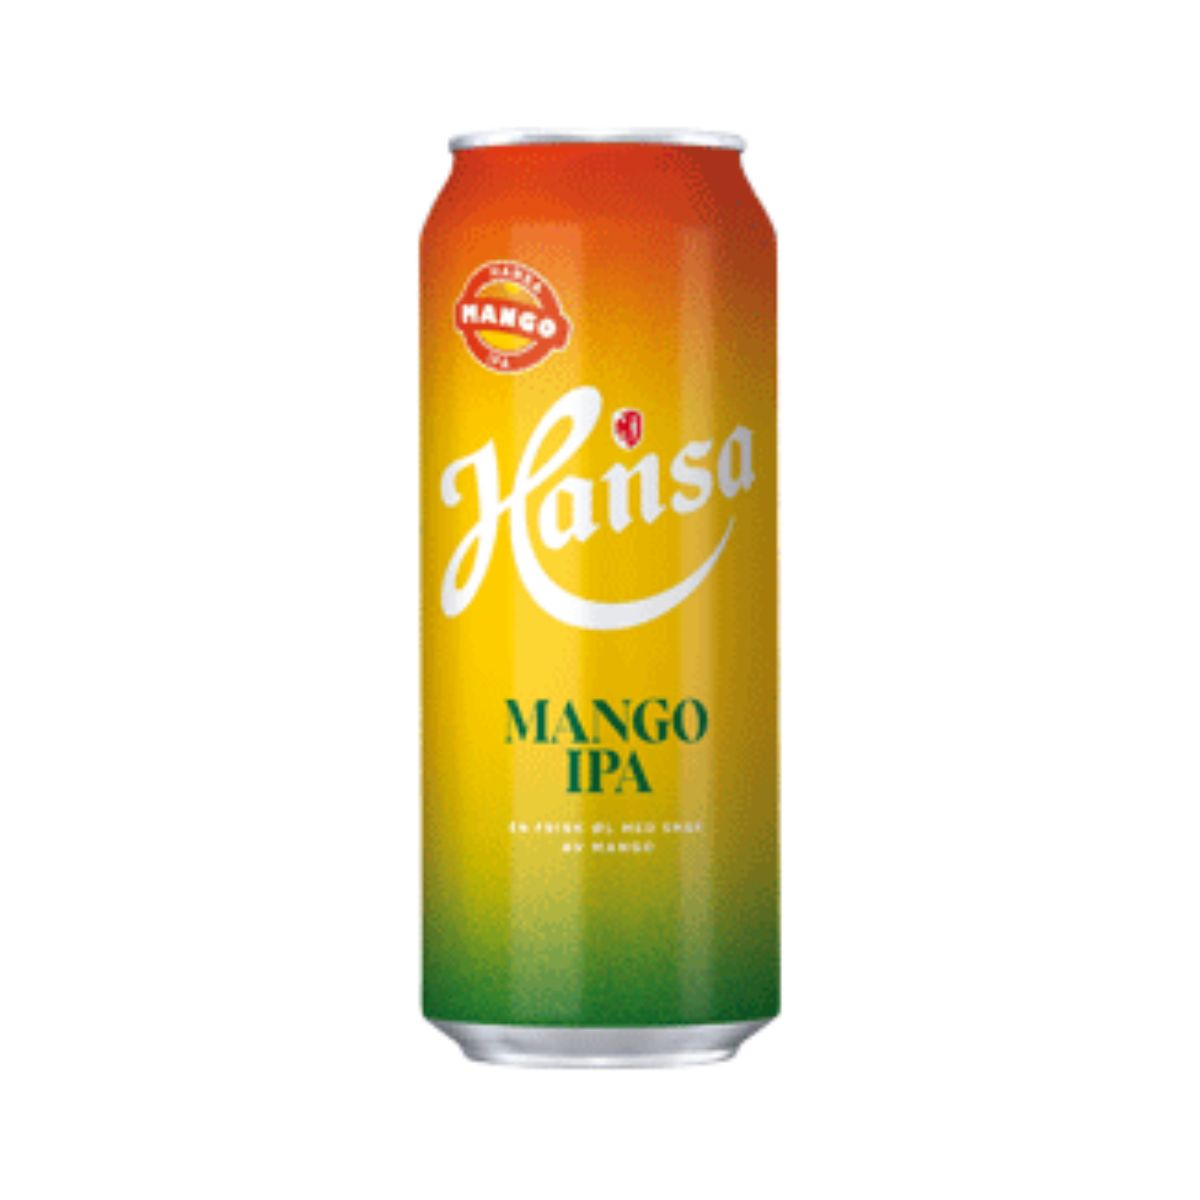
\includegraphics[width=0.5\textwidth]{Bilder/mango.jpg}
    \caption{Mango Ipa We Like}\label{fig:Mango-Logo}
\end{figure}
    